\documentclass[11pt]{article}
\usepackage[margin=1in]{geometry}
\usepackage{booktabs}
\usepackage{array}
\usepackage{amsmath}
\usepackage{amssymb}
\usepackage{graphicx}
\usepackage{listings}
\usepackage{xcolor}

\lstset{
    basicstyle=\ttfamily\small,
    breaklines=true,
    breakindent=0pt,
    frame=single,
    backgroundcolor=\color{gray!10}
}

\begin{document}
\thispagestyle{empty}

\section*{Graduate Extension: What the Constraints Induce, and Whether Closure Finds Mutants, Project 1}

\paragraph{What is analyzed.}
The team's \texttt{crv/} layer was still in progress when this was written, so
the analysis uses the constraint in \texttt{grad/stimulus.py}. It is a two-phase
sweep. In FILL, $P(\texttt{wr\_en}) = a$ and $P(\texttt{rd\_en}) = 1-a$. DRAIN
is the mirror image. At \texttt{count} $0$ and $8$ both enables are $1/2$. The
phase flips when the \emph{reference} queue reaches full or empty, and the
design value is $a = 0.75$. Every request is legal at every occupancy, because
the spec defines a write while full and a read while empty. The baseline is an
unshaped \texttt{UniformTxn}. Stimulus runs through the team's driver, monitor,
\texttt{FifoEnv} and queue scoreboard, with its own coverage phase, so no
directed cycle earns credit. The scripts accept any class with the same fields.
The tables below are regenerated when the team class lands.

\paragraph{The rates are measured, not read off the constraint.}
Each enable is an \texttt{implies} on a uniform roll. On the pinned pyvsc that
text alone does not deliver its rates. The solver picks the 1-bit enable first
and then finds a consistent roll, which pulls every rate toward $0.5$. That is
the same compression I measured in HW5. Adding
\texttt{vsc.solve\_order(roll, enable)} picks the roll first, and the rates
come back. Measured over 2000 draws per state:

\begin{table}[h]
\centering
\begin{tabular}{@{}lccc@{}}
\toprule
\textbf{state} & nominal $(p_w, p_r)$ & with \texttt{solve\_order} & same text, without \\
\midrule
$c=3$, FILL  & $(0.75, 0.25)$ & $(0.722, 0.249)$ & $(0.637, 0.396)$ \\
$c=3$, DRAIN & $(0.25, 0.75)$ & $(0.247, 0.739)$ & $(0.428, 0.662)$ \\
$c=0$ and $c=8$ & $(0.50, 0.50)$ & $(0.495, 0.514)$, $(0.499, 0.502)$ & $(0.523, 0.542)$, $(0.526, 0.530)$ \\
\bottomrule
\end{tabular}
\end{table}

\noindent
Interior drift is $+0.47$ with the ordering line and $+0.24$ without it. Every
number below comes from a chain built on the \emph{measured} joint request
probabilities, not on the constraint text.

\paragraph{The occupancy histogram, against uniform.}
Count and phase are fed in each cycle and the rolls are fresh, so stimulus is
a Markov chain on $(c, \text{phase})$, with 16 reachable states. Solving
$\pi P = \pi$ and summing out the phase gives the occupancy the constraints
induce. Figure~\ref{fig:occ} compares that prediction with the RTL histogram
from five 1024-draw seeds.

\begin{figure}[h]
\centering
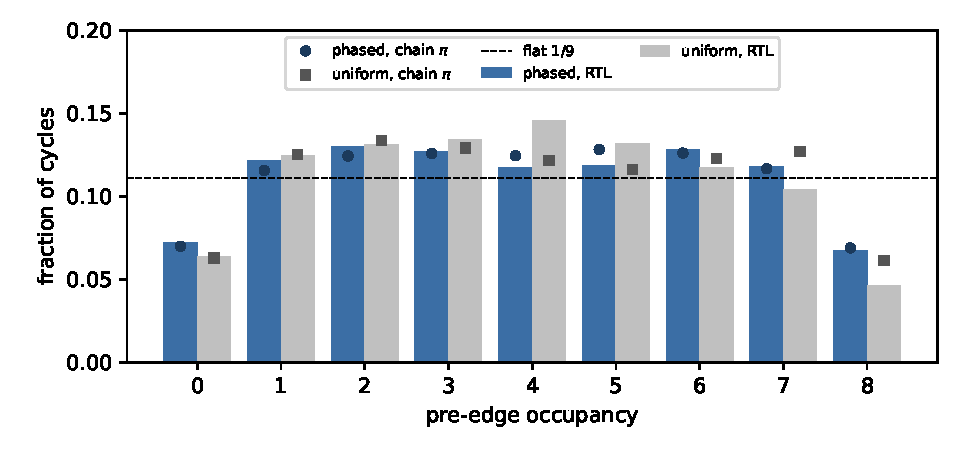
\includegraphics[width=0.82\textwidth]{figures/occupancy.pdf}
\caption{Pre-edge occupancy. Bars are RTL coverage counts over $5 \times 1024$ draws; markers are the chain's $\pi$.}
\label{fig:occ}
\end{figure}

\begin{table}[h]
\centering
\begin{tabular}{@{}lrrrrrrrrr@{}}
\toprule
$c$ & 0 & 1 & 2 & 3 & 4 & 5 & 6 & 7 & 8 \\
\midrule
phased, $\pi$   & .070 & .116 & .124 & .126 & .125 & .128 & .126 & .117 & .069 \\
phased, RTL     & .072 & .122 & .130 & .127 & .118 & .118 & .128 & .118 & .067 \\
uniform, $\pi$  & .063 & .125 & .134 & .129 & .122 & .116 & .123 & .127 & .061 \\
uniform, RTL    & .064 & .125 & .131 & .134 & .146 & .132 & .118 & .104 & .047 \\
\bottomrule
\end{tabular}
\end{table}

\noindent
The shaping barely moves the histogram. The total-variation distance between
the phased and uniform stationary distributions is $0.033$, and each is about
$0.09$ from flat. Both halve the end states for the same reason HW5 found: an
end can only be left one way. If the histogram were the only evidence, the
constraint would look like it did nothing.

One number does separate them. The phased RTL histogram is within $0.019$ TV
of its own $\pi$, and uniform is $0.046$ from its own. Uniform stimulus is a
symmetric random walk, so 5120 draws are not enough to mix. Its count-8 bar is
$0.047$ against a stationary $0.061$. What the constraint changed is the
\emph{time} structure: it crosses the FIFO in a straight line instead of
diffusing. A histogram cannot show that, so the next part measures time
directly.

\paragraph{A constraint that reaches \texttt{full} with a read.}
Name the corner $\mathcal{C}$: pre-edge $c = 8$ and \texttt{rd\_en} $= 1$ on the
same draw. It is a blocked-write and accepted-read boundary, and it covers bins
\texttt{(8, read)} and \texttt{(8, simultaneous)}. Two facts about the
constraint make it tractable. Arriving at full flips the phase to DRAIN, where
$p_r = 1/2$. The only way out of full is an accepted read, and that read is
$\mathcal{C}$. So
\[
T_{\mathcal{C}} = T_{\text{fill}} + G, \qquad G \sim \mathrm{Geom}(1/2),
\]
and $T_{\text{fill}}$ is the first passage $0 \to 8$ of a birth-death chain in
FILL. It goes up with $u = a^2$ and down with $d = (1-a)^2$ in the interior.
At $c = 0$ it goes up with $u_0 = 1/2$, because there a read is ignored and
any write advances. With $m_k$ the expected time from $k$ to $k+1$,
\[
m_0 = \frac{1}{u_0}, \qquad m_k = \frac{1 + d\, m_{k-1}}{u}, \qquad
\mathbb{E}[T_{\text{fill}}] = \sum_{k=0}^{7} m_k ,
\]
which is $16.0$ draws at $a = 0.75$, so $\mathbb{E}[T_{\mathcal{C}}] = 18$.
The expectation does not bound the tail, so the exact probability comes from
making $\mathcal{C}$ absorbing and iterating $e_0 P_{\text{abs}}^N$.

Target: $P(\mathcal{C} \text{ within } N) > p = 0.999$ for $N = 48 = 6 \cdot
\texttt{DEPTH}$ draws from reset. Sweeping $a$ on the exact chain:

\begin{table}[h]
\centering
\begin{tabular}{@{}lrrrrrrrr@{}}
\toprule
$a$ (FILL write, \%) & 66 & 68 & 70 & 71 & \textbf{72} & 73 & 74 & 75 \\
\midrule
$P(\mathcal{C}$ within 48$)$ & .9741 & .9899 & .9967 & .9982 & \textbf{.9991} & .9995 & .9998 & .9999 \\
$\mathbb{E}[T_{\text{fill}}]$ & 23.5 & 21.2 & 19.4 & 18.6 & 17.9 & 17.2 & 16.6 & 16.0 \\
\bottomrule
\end{tabular}
\end{table}

\noindent
So the derived constraint is $a \geq 0.72$ with ends at $1/2$. I use
$a = 0.75$. With the measured rates the chain gives $0.9998$ at $N = 48$, and
it crosses $0.999$ at $N = 42$. Figure~\ref{fig:corner} shows the whole curve.

\begin{table}[h]
\centering
\begin{tabular}{@{}lrrl@{}}
\toprule
\textbf{stimulus} & chain, $P_{48}$ & $N$ for $0.999$ & pyvsc, 3000 seeds, $P_{48}$ [95\% CI] \\
\midrule
phased, \texttt{solve\_order}  & .9998 & 42  & .9997 [.9981, .9999] \\
phased text, no ordering       & .8981 & 101 & .8983 [.8870, .9086] \\
uniform                        & .1934 & 751 & .2010 [.1870, .2157] \\
\bottomrule
\end{tabular}
\end{table}

\begin{figure}[h]
\centering
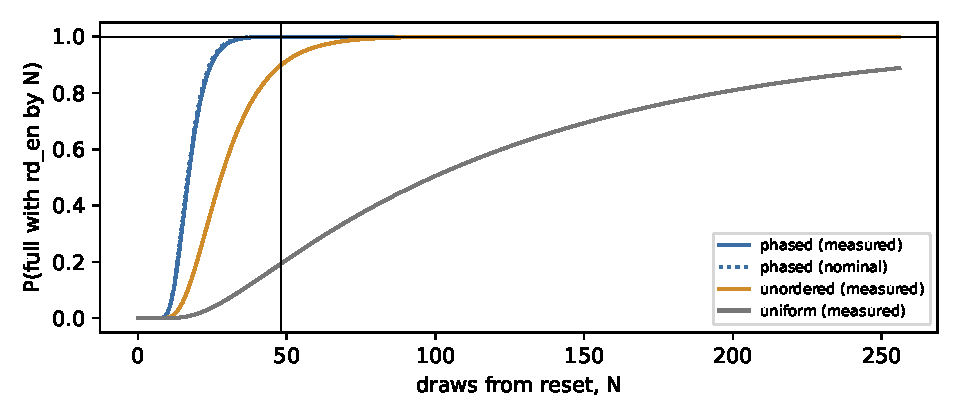
\includegraphics[width=0.75\textwidth]{figures/corner.pdf}
\caption{Exact $P(\mathcal{C}$ within $N)$ from each measured chain. The lines mark $N = 48$ and $p = 0.999$.}
\label{fig:corner}
\end{figure}

\noindent
The Monte Carlo runs pyvsc itself against the reference queue, with a fresh
transaction per seed (10000--12999). It agrees with the chain in every row, but 3000 seeds cannot tell $0.9997$ from $0.9998$; that
would need about $10^5$. The RTL regression agrees too. The phased runs hit
$\mathcal{C}$ in 3/5 seeds at $N = 16$, where the chain predicts $0.42$, and in
5/5 from $N = 32$ ($0.985$). Uniform hits it in 1/5 at 64 ($0.30$), 3/5 at 128
($0.62$), 4/5 at 256 ($0.89$), and 5/5 at 512 ($0.99$). Note the gap between
the first two rows: the \texttt{solve\_order} line alone cuts the required $N$
by $2.4\times$. And the uniform walk needs $18\times$ more draws for the
corner while spending almost the same fraction of its time at full. That is
the dwell versus traversal trade again, measured this time instead of argued.

\paragraph{Does closing holes find more mutants?}
The regression is 2 stimuli $\times$ 8 budgets ($N = 8, \dots, 1024$) $\times$ 5
seeds, 80 points in all. Each point is a clean run that exports X1 (occupancy
$\times$ request, 36 bins), then the released pool through the course harness
with identical settings. The harness reruns clean RTL first, so that is 800
simulations, and every found outcome is \texttt{test-failed}.

\begin{table}[h]
\centering
\begin{tabular}{@{}lrrrrrrrr@{}}
\toprule
$N$ & 8 & 16 & 32 & 64 & 128 & 256 & 512 & 1024 \\
\midrule
phased: mean X1 bins    & 7.8 & 13.8 & 23.8 & 29.8 & 34.0 & 36 & 36 & 36 \\
phased: mean found      & 5.0 & 6.8 & 7.6 & 7.8 & 8.0 & 8.0 & 8.0 & 8.0 \\
uniform: mean X1 bins   & 6.4 & 10.2 & 15.8 & 20.6 & 30.2 & 34.2 & 36 & 36 \\
uniform: mean found     & 5.0 & 5.8 & 6.2 & 6.4 & 7.4 & 7.8 & 8.0 & 8.0 \\
\bottomrule
\end{tabular}
\end{table}

\begin{figure}[h]
\centering
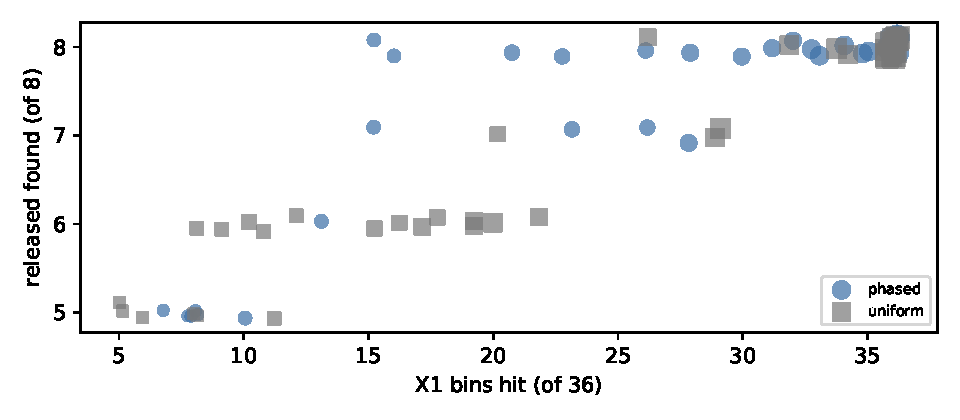
\includegraphics[width=0.75\textwidth]{figures/coverage_vs_found.pdf}
\caption{X1 bins against released found, one marker per point (jittered; size grows with $N$).}
\label{fig:cov}
\end{figure}

\noindent
Across all 80 points, Spearman $\rho = 0.87$ (Pearson $0.91$). That headline
overstates the link, for four reasons.

\begin{itemize}
\item \textbf{Closure was sufficient, not necessary.} All 29 runs that closed X1
found 8/8. But 18 runs found 8/8 with holes still open, one of them at only
15/36 bins. After a run reaches 8/8, closing its remaining holes bought nothing
on this pool.
\item \textbf{A few specific bins carry the correlation.} \texttt{ignore\_full}
was found in 47/47 runs that hit \texttt{(8, write)} or \texttt{(8,
simultaneous)}, and in 0/33 that did not. \texttt{full\_offbyone} was found in
54/54 runs that reached occupancy 7, and in 0/26 that did not. Those are the
boundary bins a diffusing walk reaches late. That is why phased reaches 8/8 at
$N = 128$ and uniform needs $N = 512$.
\item \textbf{X1 is silent on the other classes.} \texttt{empty\_offbyone},
\texttt{count\_wr\_dec}, \texttt{rd\_data\_wrptr} and \texttt{mem\_corrupt}
were found in all 80 runs, including the 8-draw ones. \texttt{ignore\_empty}
was found in 6 runs that never sampled a read at empty. The unsampled final
drain did it, so the credit belongs to the drain, not to a bin.
\texttt{wrptr\_wrap\_early} depends on the number of writes since reset, which
no X1 bin records: 0/10 at $N=8$, 8/10 at $N=16$, all from $N=32$.
\item \textbf{Both variables grow with $N$.} Within a single budget, $\rho$ is
$0.71$ to $0.85$ for $N = 16$ to $256$. That mostly separates phased from
uniform at the same $N$, which is the boundary-bin mechanism above, not
evidence that bins in general predict detection.
\end{itemize}

\noindent
So the answer is yes, for the holes a mutant's activation condition actually
lives in. It is no for the cross as a whole. Closure is a useful sign-off
check because it forces the boundary bins, but the queue scoreboard, the drain
and traversal count are what found the other half of the pool. For the team
suite this argues for a pointer-wrap coverpoint (writes since reset, in units
of \texttt{DEPTH}) next to X1. Any fault class that X1 cannot see will not
show up in this correlation either.

\paragraph{Limits.}
Five seeds per point. The released pool has eight mutants, and the hidden pool
may weight the classes differently. WIDTH and DEPTH are both 8. The constraint
analyzed is the extension's own, not the team's final \texttt{crv/} class.
Commands, seeds and per-run stream hashes are in \texttt{grad/README.md} and
\texttt{grad/results/}. All 80 streams are distinct. Rerunning
\texttt{analyze.py} reproduces \texttt{analysis.json} byte for byte, and
Monte Carlo trials rerun alone match the loop (\texttt{mc\_reproduce.log}).

\section*{AI Assistance Disclosure}

I used a general-purpose frontier assistant, terminal interface, to implement
the analysis scripts, run the regression, and draft this write-up. Every
number is taken from the logged results in \texttt{grad/results/}. The
predictions, evidence and fixes are recorded in \texttt{ai\_log.md}, including a
Monte Carlo seeding bug a teammate's review caught. The prompt:

\begin{lstlisting}
"Help me complete my portion of my verification/validation group project ... Also help me complete the graduate extension as a latex file ... Make sure to include AI disclosures where appropriate."
\end{lstlisting}

\noindent
Accessed on 10/31/26 and 11/4/26.

\end{document}
